\PassOptionsToPackage{table}{xcolor}
\documentclass[12pt,letterpaper,twocolumn,openany,nodeprecatedcode,bg=none]{dndbook}
\usepackage[english]{babel}
\usepackage[utf8]{inputenc}
\usepackage{longtable,booktabs,array}
\usepackage{calc}
\usepackage{etoolbox}
\usepackage{caption}
\usepackage{float}
\usepackage{graphicx}
\usepackage{needspace}
\usepackage{tikz}

% Reset zebra striping at the start of every table
\AtBeginEnvironment{longtable}{\rowcolors{1}{white}{gray!10}\small}
\AtBeginEnvironment{table}{\rowcolors{1}{white}{gray!10}}

\providecommand{\pandocbounded}[1]{#1}
\providecommand{\tightlist}{%
  \setlength{\itemsep}{0pt}\setlength{\parskip}{0pt}}

\captionsetup{labelformat=empty}
\setcounter{secnumdepth}{0}
\setlength{\parindent}{0pt}
\setlength{\parskip}{0.5\baselineskip}
\setlength{\headheight}{15pt}

% Prevent orphaned subsections
\let\oldsubsection\subsection
\renewcommand{\subsection}[1]{%
  \needspace{5\baselineskip}%
  \oldsubsection{#1}%
}

\begin{document}
\onecolumn

      \title{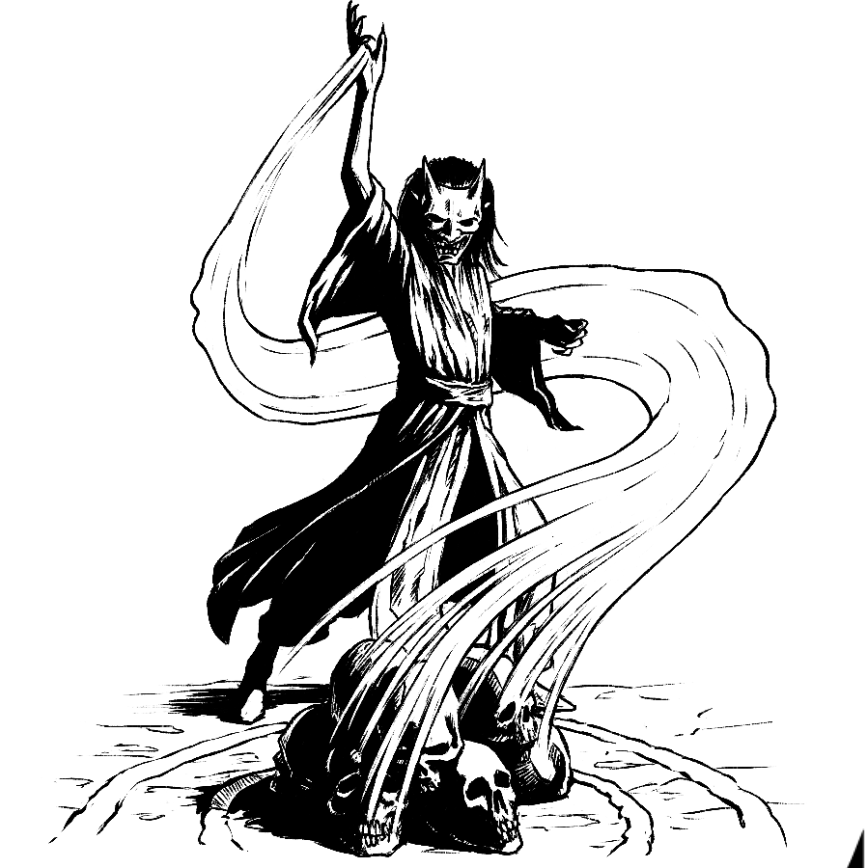
\includegraphics[width=0.9\textwidth,height=0.55\textheight,keepaspectratio]{necromancer.png}\\[1.5cm]Necromancer}
  \author{Class Handbook}
\date{}
\maketitle


\clearpage
\thispagestyle{empty}
\begin{center}
\vspace*{\fill}
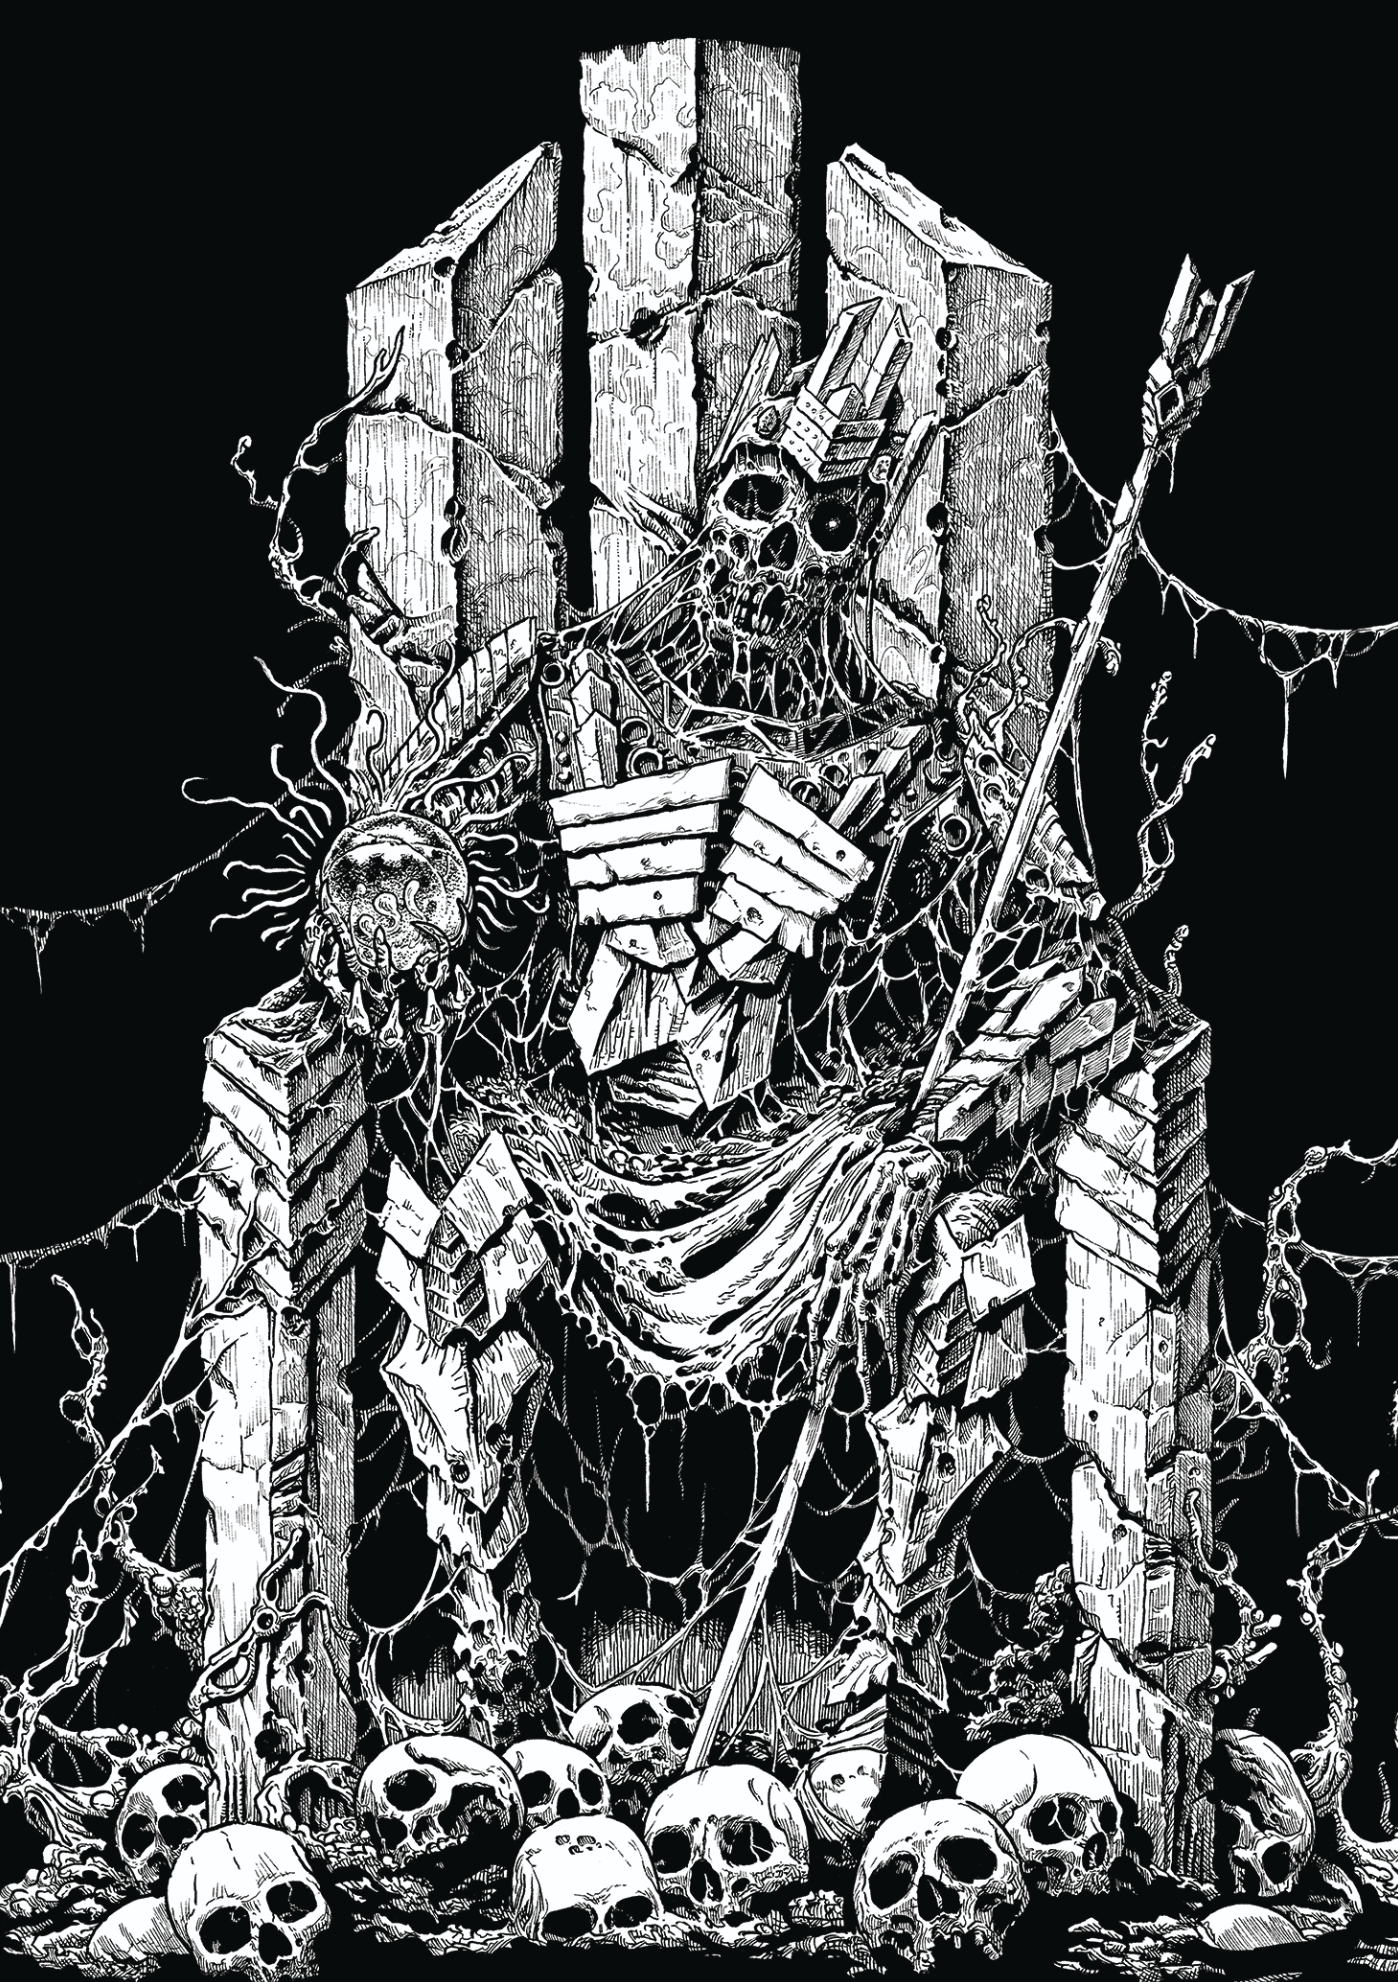
\includegraphics[width=\textwidth,height=0.85\textheight,keepaspectratio]{lich.png}\par
\vspace{0.4cm}
{\itshape The ultimate goal of any necromancer is to ascend to
lichdom.}\par
\vspace*{\fill}
\end{center}

\clearpage
\twocolumn

\section{Necromancer}\label{necromancer}

\subsection{Core Necromancer Traits}\label{core-necromancer-traits}

\needspace{11\baselineskip}

{\def\LTcaptype{none} % do not increment counter
\begin{table}[!htbp]
\centering
\begin{tabular}{@{}
  >{\raggedright\arraybackslash}p{(\linewidth - 2\tabcolsep) * \real{0.4127}}
  >{\raggedright\arraybackslash}p{(\linewidth - 2\tabcolsep) * \real{0.5873}}@{}}
\toprule\noalign{}
\begin{minipage}[b]{\linewidth}\raggedright
\textbf{Primary Ability}
\end{minipage} & \begin{minipage}[b]{\linewidth}\raggedright
Intelligence
\end{minipage} \\
\midrule\noalign{}
\textbf{Hit Points} & 1d6 \\
\textbf{Saving Throw Proficiencies} & Intelligence, Wisdom \\
\textbf{Skill Proficiencies} & Choose 2 skills \\
\textbf{Weapon Proficiencies} & Choose 1 category \\
\textbf{Starting Equipment} & Padded Jacket, Grimoire, Robe, Dagger \\
\bottomrule\noalign{}
\end{tabular}
\end{table}
}

\subsection{Necromancer Features}\label{necromancer-features}

\needspace{20\baselineskip}

{\def\LTcaptype{none} % do not increment counter
\begin{table}[!htbp]
\centering
\begin{tabular}{@{}
  >{\raggedright\arraybackslash}p{(\linewidth - 8\tabcolsep) * \real{0.0769}}
  >{\raggedright\arraybackslash}p{(\linewidth - 8\tabcolsep) * \real{0.1692}}
  >{\raggedright\arraybackslash}p{(\linewidth - 8\tabcolsep) * \real{0.1077}}
  >{\raggedright\arraybackslash}p{(\linewidth - 8\tabcolsep) * \real{0.0769}}
  >{\raggedright\arraybackslash}p{(\linewidth - 8\tabcolsep) * \real{0.5692}}@{}}
\toprule\noalign{}
\begin{minipage}[b]{\linewidth}\raggedright
Level
\end{minipage} & \begin{minipage}[b]{\linewidth}\raggedright
Proficiency
\end{minipage} & \begin{minipage}[b]{\linewidth}\raggedright
Rituals
\end{minipage} & \begin{minipage}[b]{\linewidth}\raggedright
Tools
\end{minipage} & \begin{minipage}[b]{\linewidth}\raggedright
Class Features
\end{minipage} \\
\midrule\noalign{}
1 & +2 & 1 & 2 & Apprentice of Undeath, Tools of Death \\
2 & +2 & 1 & 2 & --- \\
3 & +2 & 1 & 2 & Ability Bonus \\
4 & +2 & 2 & 2 & --- \\
5 & +2 & 2 & 3 & Death's Harvest \\
6 & +2 & 2 & 3 & --- \\
7 & +2 & 3 & 3 & Ability Bonus \\
8 & +2 & 3 & 3 & --- \\
9 & +3 & 3 & 3 & --- \\
10 & +3 & 3 & 3 & Endless Undeath \\
\bottomrule\noalign{}
\end{tabular}
\end{table}
}

The \textbf{Rituals} column shows how many rituals you know. The
\textbf{Tools} column shows how many tools of death you carry. Both
increase automatically as shown.

\subsection{Level 1: Apprentice of
Undeath}\label{level-1-apprentice-of-undeath}

You have learned to breach the barrier between life and death,
commanding the dead to serve you.

\textbf{Saving Throws.} The saving throw DC of your necromancer features
is 8 + your Intelligence modifier + your proficiency bonus.

\textbf{Rituals.} You master blasphemous rituals that animate the dead
or call forth spirits. Each ritual has a level and your level must be
greater than or equal to its level to take it. When you gain a level,
you can replace one ritual you know with another.

\textbf{Controlling the Dead.} Each summoned undead has a stat block,
including the initiative it acts on (undead do not roll initiative).
When you summon an undead, it appears within 30 feet of you and obeys a
general command you issue. Undead can perform any task you can describe,
but lack specialized knowledge or creativity. They cannot craft new
things or work autonomously.

\textbf{Soul Focus.} When you use a ritual to create undead, that ritual
requires your soul focus. The next time you use another ritual, the
ritual that needed your soul focus ends. You can only have one soul
focus ritual active at a time.

\subsection{Level 1: Tools of Death}\label{level-1-tools-of-death}

Your ability to pierce the veil allows you to craft objects infused with
death energy. You gain two tools of death of your choice from the list
at the end of this class.

If you lose a tool, you can craft a replacement as part of a long rest;
the item is ready when the rest ends. You can replace one tool each long
rest.

\textbf{Dark Arts.} If you use your action to use a ritual, you can also
use a tool of death that turn without using an additional action.

\subsection{Level 3: Ability Bonus}\label{level-3-ability-bonus}

You gain a +1 bonus to two abilities of your choice.

\subsection{Level 5: Death's Harvest}\label{level-5-deaths-harvest}

Once per turn when a creature within 30 feet of you dies, you regain hit
points equal to your Intelligence modifier.

\subsection{Level 7: Ability Bonus}\label{level-7-ability-bonus}

You gain a +1 bonus to two abilities of your choice.

\subsection{Level 10: Endless Undeath}\label{level-10-endless-undeath}

At the start of your turn, any undead created by your currently active
soul focus ritual that were destroyed return to unlife with full hit
points.

\newpage

\section{Rituals}\label{rituals}

Rituals that require your soul focus note that in their duration entry.

\subsection{Animate Zombies}\label{animate-zombies}

\textbf{Level:} 1 Ritual (Necromancer)

\textbf{Casting Time:} 1 action

\textbf{Range:} 30 feet

\textbf{Duration:} Permanent (Soul Focus)

You call forth spirits of the dead to animate nearby corpses up to size
Medium. If you invoke this ritual and already have zombies animated with
it, you animate additional ones until you reach your limit. You animate
one zombie at level 1, two at level 5, and three at level 9.

\textbf{AC} 12 --- \textbf{HP} 12 --- \textbf{Tests} +0 (Str, Con +2)
--- 30 feet

\textbf{Death Proof (15+).} When reduced to 0 hit points by damage other
than radiant, roll a d20. On 15+ it is instead reduced to 1 hit point.

\textbf{Initiative 5: Rend and Tear.} Melee attack with attack bonus of
your proficiency + Intelligence modifier. \textbf{Hit:} 1d8 bludgeoning
damage.

\newpage

\subsection{Animate Skeletons}\label{animate-skeletons}

\textbf{Level:} 3 Ritual (Necromancer)

\textbf{Casting Time:} 1 action

\textbf{Range:} 30 feet

\textbf{Duration:} Permanent (Soul Focus)

You conjure forth the spirits of slain warriors to animate skeletons up
to size Medium. If you invoke this ritual and already have skeletons
animated with it, you animate additional ones until you reach your
limit. You animate one skeleton at level 3, two at level 6, and three at
level 10.

\textbf{AC} 16 --- \textbf{HP} 8 --- \textbf{Tests} +0 (Dex +2) --- 30
feet

\textbf{Death Splinters.} If killed by a melee attack, the creature that
destroyed it takes 1d8 piercing damage.

\textbf{Initiative 20: Slashing Claws.} Melee attack with attack bonus
of your proficiency + Intelligence modifier. \textbf{Hit:} 1d6 slashing
damage.

\subsection{Call Wrathful Ghost}\label{call-wrathful-ghost}

\textbf{Level:} 7 Ritual (Necromancer)

\textbf{Casting Time:} 1 action

\textbf{Range:} 30 feet

\textbf{Duration:} Permanent (Soul Focus)

You draw the ghost of someone who died a painful death. The spirit
manifests using the stats below.

\textbf{AC} 13 --- \textbf{HP} 25 --- \textbf{Tests} +1 (Cha +4) --- 40
feet (Fly)

\textbf{Incorporeal.} Can move through but cannot end a turn inside a
solid object.

\textbf{Insubstantial (16+).} The first time this creature takes damage
on a turn, roll a d20. On 16+ it takes no damage that turn.

\textbf{Initiative 10: Frightening Howl.} Hostile creatures in melee
range must make a Wisdom save using necromancer's save DC.
\textbf{Failure:} 1d4 psychic damage per 2 necromancer levels, and
frightened of the ghost for 1 round. \textbf{Success:} Half damage

\subsection{Curse of Death's Doorstep}\label{curse-of-deaths-doorstep}

\textbf{Level:} 10 Ritual (Necromancer)

\textbf{Casting Time:} 1 action

\textbf{Range:} 120 feet

\textbf{Target:} 1 creature

\textbf{Duration:} 3 rounds

You weave necromantic energy through a creature's spirit, sending
tendrils into the future to draw its death hurtling toward it. The
target creature gains a death curse, its life energy bleeding away each
time death comes to call. Once per round when a creature within 30 feet
of it dies, it takes 3d12 necrotic damage.

\subsection{Gaze of the Bloody Skull}\label{gaze-of-the-bloody-skull}

\textbf{Level:} 7 Ritual (Necromancer)

\textbf{Casting Time:} 1 action

\textbf{Range:} 30 feet

\textbf{Duration:} 1 round

The skin covering your skull peels back, revealing a horrid, bloody mask
that leaves creatures shrieking in terror. Creatures of your choice
within 30 feet of you must make Wisdom saves. On a failed save, a
creature is frightened of you and cannot move closer to you.

\subsection{Vampiric Harvest}\label{vampiric-harvest}

\textbf{Level:} 1 Ritual (Necromancer)

\textbf{Casting Time:} 1 action

\textbf{Range:} 120 feet

\textbf{Target:} 1 creature

\textbf{Duration:} 1 round

You infuse an aura of death energy around a creature, allowing you to
collect its life energy and share it with an ally.

Once per turn when the target takes damage, you gain one blood point. At
the start of your next turn when the spell's duration expires, a
creature of your choice within range regains 3 hit points per blood
point you collected. You then lose all blood points.

\newpage

\section{Tools of Death}\label{tools-of-death}

\subsection{Death Mask}\label{death-mask}

You weave a ghoulish mask from skin taken from an embalmed corpse. When
you wear the mask you gain the following benefits.

When making Charisma checks to influence undead creatures, add your
Intelligence modifier as a bonus to the roll.

As a magic attack action, you can stare at a creature within 120 feet
and fill it with dread. It must make a Wisdom save. On a failed save, it
is frightened of you for one round and takes psychic damage based on
your level.

The damage is 1d4 at level 1, 2d4 at level 5, and 3d4 at level 10.

\subsection{Death-Eyed Skull}\label{death-eyed-skull}

You collect a skull and scribe it with blasphemous runes of death and
annihilation. You can present the skull and channel power through it,
causing a sickly beam of crimson energy to emit from it as a magic
attack action. This is an attack against one target with a range of 120
feet that uses your Intelligence modifier on its attack and damage
rolls. On a hit, the target comes under a death curse and suffers
psychic damage based on your level. While cursed, undead creatures have
advantage on attacks against it for one round.

The damage is 1d4 at level 1, 2d4 at level 5, and 3d4 at level 10.

\subsection{Emissary Skull}\label{emissary-skull}

You have the skull of a linguist and ambassador. Treated with runes, it
retains a shadow of its former knowledge.

If the skull is daubed with blood or other remains taken from a slain
creature, it gains the knowledge of all languages that creature speaks.
You can speak, understand, and read those languages while you hold the
skull. If you use this ability again, the skull loses the prior
languages it learned, replacing them with the new ones.

\subsection{Scythe of Reaping}\label{scythe-of-reaping}

You imbue a scythe with the energies that simmer between life and death.
It becomes a cutting tool that you can use to reap life energy from your
enemies. The scythe is a two-handed, reach melee weapon that does 1d6
slashing damage.

In your hands, the weapon uses your Intelligence modifier for its attack
and damage bonus.

At higher levels, you gain reaper dice as the scythe's cuts open the
gate between life and death. Your reaper dice are 1d6 at level 5, 2d6 at
level 7, and 3d6 at level 10.

When you hit a hostile creature with the scythe, you can roll the reaper
dice and apply the total as necrotic damage to the target of your attack
or as healing to a creature within melee range of you.

\subsection{Thief's Hands}\label{thiefs-hands}

You have acquired the severed hands of a dead thief and, with your
magic, have imbued the thief's cunning into them.

The hands are two Tiny objects with AC 15, 2 hit points each, and a test
bonus equal to your Intelligence modifier + your proficiency bonus. They
have advantage on all Stealth checks. They have a climb speed.

As an action, you can direct them to open doors, search through treasure
piles, and take other actions as you direct. As a search action, you can
project your senses through one of them, allowing you to see and hear
everything it senses for one round.

The hands understand how to use lock picks and can be directed to pick
locks and disable traps if they are carrying the appropriate tools.

\onecolumn

\clearpage
\thispagestyle{empty}
\begin{center}
\vspace*{\fill}

\includegraphics[width=0.7\textwidth,keepaspectratio]{skull.png}\par
\vspace{0.4cm}
{\itshape The skull is the most ancient and feared symbol of
necromancy.}\par
\vspace*{\fill}
\end{center}

\end{document}